%*********************第五章******************
\chapter{面向卷积神经网络前向过程的低延迟实现}
\section{引言}
随着卷积神经网络应用的越来越广泛,数据中心开始需要为用户提供神经网络前向计算过程的服务,而用户希望数据中心能够尽快响应,因此,在数据中心部署一个满足低延迟前向过程的神经网络具有重要的意义。特别是随着神经网络结构变得更深更复杂,处理的应用也由2D变为3D,所需的计算量不断地在增长,低延迟就更加重要了。而现有的数据中心一般都是拥有大量的计算资源,这为加速神经网络前向计算过程提供了硬件基础。针对数据中心大量的硬件计算资源,如何发挥计算资源的效能并且满足用户的低延迟需求变得尤为重要。对于神经网络的训练来说,用户不会有低延迟的需求,但对于神经网络的前向推测过程,用户是非常关注延迟的。神经网络的训练中采用的并行方法对于神经网络的前向推测过程就不适用了。神经网络的训练是以批处理的方式进行训练的,一次处理大量的输入,为了减少计算过程间的通信,一般采用数据并行的方式。而神经网络的前向推测过程一般需要立即处理用户提交的单个输入,虽然有多个计算设备,但却无法采用训练中数据并行的方式进行加速,而需采用模型并行的方法才能达到低延迟的目标。模型并行是将模型参数分割在多个计算设备,这也可以解决模型参数过大在单个设备存储不足的问题,此外,神经网络每一层网络的计算都是由多个计算设备一起完成的,在每一层计算结束之后,各个计算设备间需要通信进行数据交换。

本章的目的主要是在数据中心环境下解决神经网络前向推测过程的低延迟问题。其中涉及到在多个计算设备上并行加速的问题,本章主要介绍如何采用模型并行的技术来对神经网络进行加速计算,并对模型并行中涉及到的通信问题,采用CUDA-Aware MPI技术使得GPU间通信更加高效,并且对多个计算设备间的通信模式进行了优化,使得通信代价不会随着计算设备的增多而增大。最后采用计算与通信进行重叠计算的技术进一步提升性能,这需要对模型并行进行流水化处理。

本章内容安排如下:第二节将介绍针对神经网络加速的相关研究,有针对算法的改进进行加速的方法,也有面向多设备采用数据并行和模型并行方法的相关研究;第三节主要介绍了关于数据并行、模型并行以及GPU间高效通信的CUDA-Aware MPI接口;第四节将主要介绍模型并行的流水化,具体包括模型并行的流水化实现,优化的通信模式设计以及计算与通信重叠的执行;最后一节将介绍实验部分,主要是2D以及3D卷积层的模型并行性能的测试。

\section{相关研究}
\label{relatedwork}
本章处理的神经网络为卷积神经网络,卷积神经网络的计算集中在卷积层,下面主要介绍针对卷积计算的加速的相关研究。首先是卷积算法的改进,Mathieu等人采用傅立叶变换的方法\upcite{mathieu2013fast}实现卷积计算,这种方法在卷积核大小比较大的时候优势明显,因为卷积核大小在一定范围内变化时,比如3~16,傅立叶方法所需的计算量不会随着卷积核大小变化而变化,而对于传统卷积方法来说,卷积核越大意味着卷积所需的计算量越大,因此,在卷积核比较大时,选择傅立叶方法在计算量方面有明显的优势,而傅立叶方法存在的问题就是所需的存储开销大,这成为限制傅立叶方法普遍使用的重要障碍。Lavin等人\upcite{lavin2016fast}将一个称为Winograd的算法应用在2D卷积计算中,并且在GPU平台上高效地实现了Winograd算法。Winograd算法是传统卷积计算方法与傅立叶方法的一种折中,即在保持存储开销不变的条件下降低计算量,最后的实验结果也表明,他们在GPU上的高效实现最后性能超过目前最快的cuDNN库。Winograd算法也非常适合在硬件加速平台上实现,Aydonat等人\upcite{aydonat2017opencl}就将Winograd算法在FPGA平台上采用高级语言进行了实现。不过这些Winograd算法的实现目前还只针对2D卷积网络。

另一种加速卷积网络计算的思路是将其中的浮点计算转化为代价更小的计算类型。比如将32位的浮点运算转化为16位浮点或者8位浮点运算,而这基本不会影响结果的精度。有些工作比如\upcite{courbariaux2015binaryconnect}、\upcite{courbariaux2016binarized}甚至将卷积计算的输入和模型参数转化为4位或者2位。而Rastegari等人\upcite{rastegari2016xnor}提出了一个XNOR网络,这个网络的输入和模型参数都是用1位来表示,而它们之间的计算则转化为异或计算,这些方法不但简化了计算而且还节省了存储开销,但存在精度下降的问题。

以上研究都还集中在单设备上对神经网络进行加速。Alex等人\upcite{krizhevsky2014one}针对神经网络的训练提出了一个混合并行的方法,这个方法主要是用在多GPU设备上,他们根据神经网络的特点,比如卷积层计算量比较大,模型参数比较少,因此,针对卷积神经网络的卷积层使用数据并行的方式,而对于卷积神经网络的全连接层,由于全连接层参数规模较大,采用模型并行的方式,这种混合并行的方式可以有效减少数据通信。在对神经网络的训练中,Awan等人专门提出了S-Caffe\upcite{awan2017s},S-Caffe采用了计算与通信重叠的技术对多GPU间的通信进行了优化。本章工作提出了流水化的模型并行方式,这对神经网络的前向计算过程具有很好的加速效果,此外,本章对模型并行中的通信优化进行了介绍。

\section{数据并行、模型并行以及CUDA-Aware MPI}
本节将介绍在神经网络中常用的两种并行方式,数据并行和模型并行,此外,本章还将介绍在多GPU间高效通信使用的CUDA-Aware MPI 进行介绍。

\subsection{数据并行与模型并行}
多GPU环境下,存在两种并行方式对卷积神经网络进行加速,即数据并行和模型并行。在数据并行中,所有的工作线程的计算过程一样,每个工作线程独立地处理不同的输入,因此数据并行方式可以有效地增加处理输入的吞吐率。对于模型并行来说,每一层卷积的模型参数都被分割到不同的计算设备中,然后每一个工作线程都只负责部分结果的计算,计算结束后,所有工作线程之间需要交换计算的结果,计算设备越多,意味着所需的通信也越多。但由于所有的计算设备同时处理卷积神经网络的每一层计算,所以,模型并行可以显著降低卷积神经网络前向推测过程的延迟,并且针对大型的卷积神经网络,由于模型参数分布在不同的计算设备中,可以解决单个设备无法存储所有模型参数的问题。图\ref{dataAndModelParallel}为数据并行与模型并行的示意图。


\begin{figure*}[tbh]%\small
\centering
%\resizebox{0.5\textwidth}{!}{
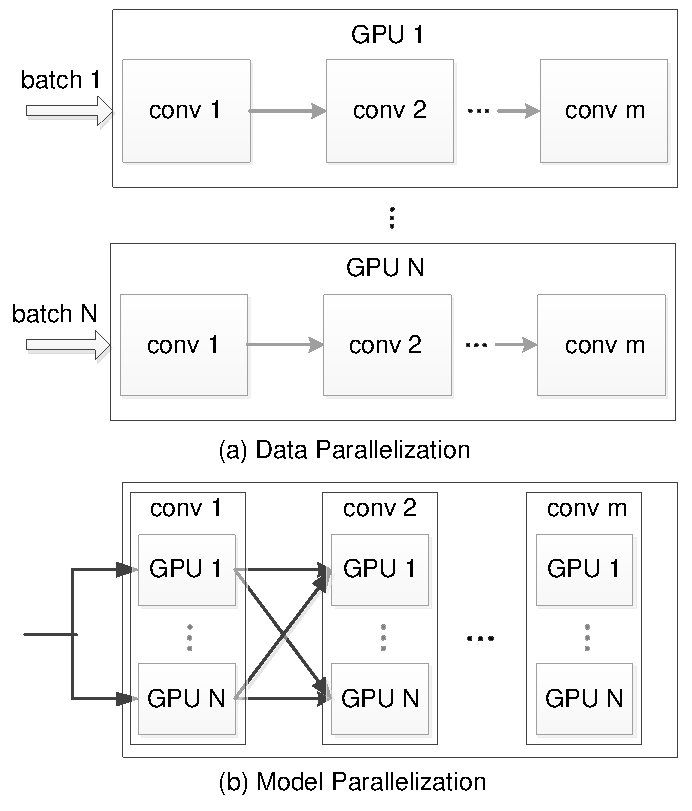
\includegraphics[width=10cm]{figs/dataAndModelParall.pdf}
%}
\caption{数据并行与模型并行.}
\label{dataAndModelParallel}
\end{figure*}

\subsection{CUDA-Aware MPI}
英伟达公司提供的GPUDirect技术使得读写GPU设备存储和主机存储变得更加直接和高效,可以减少很多不必要的数据拷贝,显著地降低CPU开销以及减少访存延迟。基于GPUDirect技术,英伟达公司在2011年更是提供了GPUDirect P2P支持,使得处于同一PCI-E连接下的GPU设备间可以相互访问各自的显存,如图\ref{GPUDirectP2P}所示,图中左边表示GPU间数据传输需要经过CPU,数据首先从GPU显存传输到CPU的主存,然后。而后面提出的GPUDirect DMA技术则解决了CPU主存与GPU显存间高效数据传输的问题。
\begin{figure*}[tbh]%\small
\centering
%\resizebox{0.5\textwidth}{!}{
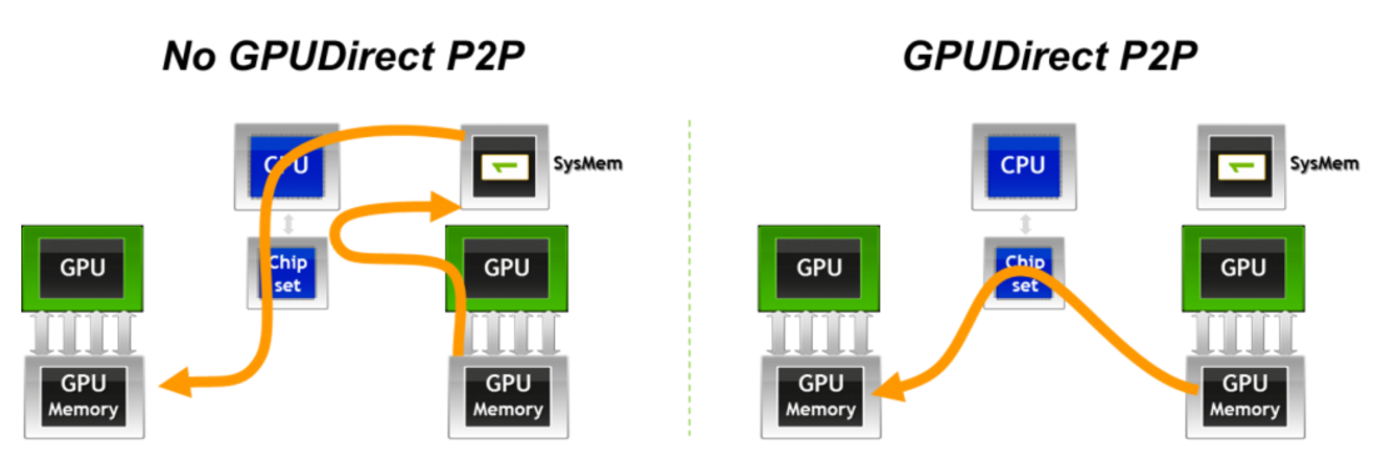
\includegraphics[width=12cm]{figs/GPUDirectP2P.pdf}
%}
\caption{GPU间数据传输的两种方式\upcite{cudaAwareMPI}。}
\label{GPUDirectP2P}
\end{figure*}

对于单节点内多GPU的异构平台,可以采用多线程的方式对各个GPU进行控制,GPU之间的通信将分两步完成,比如需要将GPU A的显存数据传输到GPU B显存中,控制GPU A的线程首先将数据从GPU A拷贝到CPU 主存中,然后控制GPU B的线程将数据从CPU的主存拷贝到GPU B的显存中。线程这种显式控制数据传输的方式虽然很直接,但程序的移植性不够好,当异构节点中GPU数量变化时,程序就需要改写。下面将介绍我们所采用的编程方式即MPI编程,MPI编程最开始运用在多节点环境下,节点间是对等的关系,针对单个节点内多GPU情形下,也同样可以创建多个MPI进程,每个MPI进程控制一个GPU,GPU间通信通过MPI进程间通信实现。而自从Nvidia支持统一虚拟地址(UVA)以及GPUDirect技术之后,通过MPI编程控制GPU间通信变得更加简单和高效,图\ref{UVA}为统一虚拟地址的示意图,统一虚拟地址空间是将CPU主存以及各个GPU的显存统一编址,各个设备的存储地址对应一段特定的空间。基于UVA和GPUDirect技术,无论是现在的OpenMPI还是MVAPICH2都支持CUDA-Aware MPI原语,所谓的CUDA-Aware MPI原语是能识别CPU主存和GPU显存从而自动完成底层硬件通信通路的最优选择,所以CUDA-Aware MPI不但编程简单,而且也是通信最高效的一种编程方法。图\ref{cuda-aware-MPI}为CUDA-Aware MPI的示意图,图中下面的通信链路代表传统的需要经过CPU控制的数据通信,上面是基于GPUDirect技术的MPI直接通信方式。此外,CUDA-Aware MPI还支持非阻塞通信,这为计算与通信重叠的使用提供基础。
\begin{figure*}[tbh]%\small
\centering
%\resizebox{0.5\textwidth}{!}{
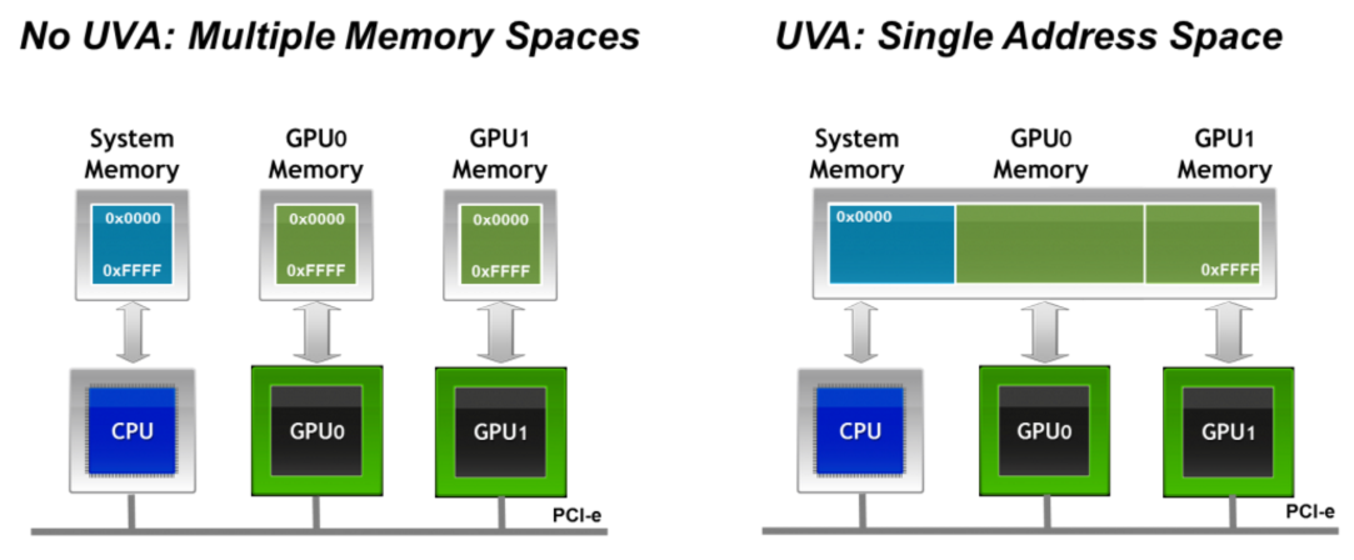
\includegraphics[width=12cm]{figs/UVA.pdf}
%}
\caption{UVA与非UVA示意图\upcite{cudaAwareMPI}。}
\label{UVA}
\end{figure*}

\begin{figure*}[tbh]%\small
\centering
%\resizebox{0.5\textwidth}{!}{
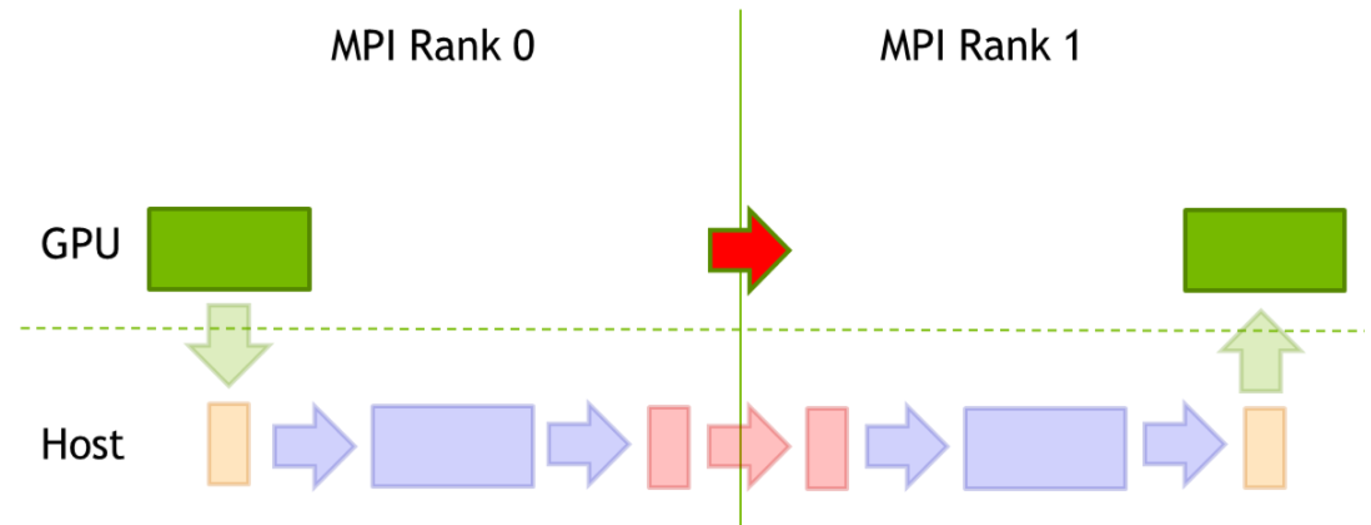
\includegraphics[width=12cm]{figs/CUDA-AwareMPI.pdf}
%}
\caption{基于GPUDirect技术的CUDA-Aware MPI通信\upcite{cudaAwareMPI}。}
\label{cuda-aware-MPI}
\end{figure*}

\section{模型并行优化}
这一节将介绍模型并行的简单实现以及模型并行的流水化实现。模型并行的简单实现只是将原来在单个GPU执行的卷积运算通过模型并行在多个GPU上实现,简单的模型并行实现分成两阶段,第一阶段是计算,第二阶段是通信;模型并行的流水化实现就是将计算分割成很多小的计算任务,在每个小的计算任务完成后进行一次通信,计算和通信交替地进行,第i次计算任务后的通信可以与第i+1次计算任务并行的执行,这就是模型并行的流水化实现。流水化的执行可以对通信进行隐藏,降低通信开销。本章还会介绍一种优化的通信模式,这种通信模式不会随着计算设备的增多而增加通信的代价。

\subsection{模型并行的简单实现}
前面已经介绍了关于模型并行的概念,我们主要将模型并行应用到卷积神经网络的卷积层,本节将介绍模型并行的简单实现。

单计算设备的卷积层实现不涉及通信过程,只包含计算过程,卷积计算的实现可以采用目前流行的库,比如cublas或者cuDNN(针对GPU平台)。多计算设备的模型并行实现,包含计算和通信两个过程,模型并行将计算任务分配到多个计算设备中,每个计算设备负责部分卷积计算,计算完成后,每个设备的计算结果需要传输到其它计算设备中。在模型并行中,虽然卷积计算被划分成多个小的计算任务,但每个小计算任务仍然属于卷积计算,因此在模型并行中,每个计算设备上的卷积计算仍然可以调用现有的库来实现,实现的关键是为每个计算设备准备好所需的数据。卷积计算涉及到输入和卷积核,经过计算最后得到卷积计算结果,在模型并行中,各个计算设备的输入都相同,而卷积核参数被划分到不同的计算设备中,最后每个计算设备的计算结果需要合并成一个计算结果,然后同步到所有计算设备中,作为下一层的输入。所以,模型并行很重要一点就是数据的存储顺序,首先是卷积核参数的划分可以直接连续地划分到各个计算设备中,其次就是各个计算设备的计算结果在合并中,可以很直接拼接在一起。

下面假定卷积层的输入的batch大小为$N$,输入的通道数为$C$,输入特征的高为$H$,宽为$W$,输入维度可表示为$N\times H\times W\times C$,卷积核的大小为$f$,输出通道数为$K$,则卷积核的维度可表示为$C\times f\times f\times K$,卷积时的步长为1,则输出的特征图的维度可表示为$N\times P\times Q\times K$。为了使模型并行时存储连续,对卷积核参数存储,需要保证最后存储的是K所在的维度,而输入的存储需要保证最后存储的是C所在的维度。模型并行中假定所使用的计算设备个数为$n$,则输入保持不变,各个计算设备的卷积核参数维度变为$C\times f\times f\times$ $\frac{K}{n}$,输出的维度变为$N\times P\times Q\times$ $\frac{K}{n}$。划分之后的任务在各个计算设备中仍然可以作为一个完整的卷积层计算,只是规模变小了。图\ref{modelparallel}为卷积层单GPU计算处理过程与双GPU模型并行的计算过程。

\begin{figure*}[tbh]%\small
\centering
%\resizebox{0.5\textwidth}{!}{
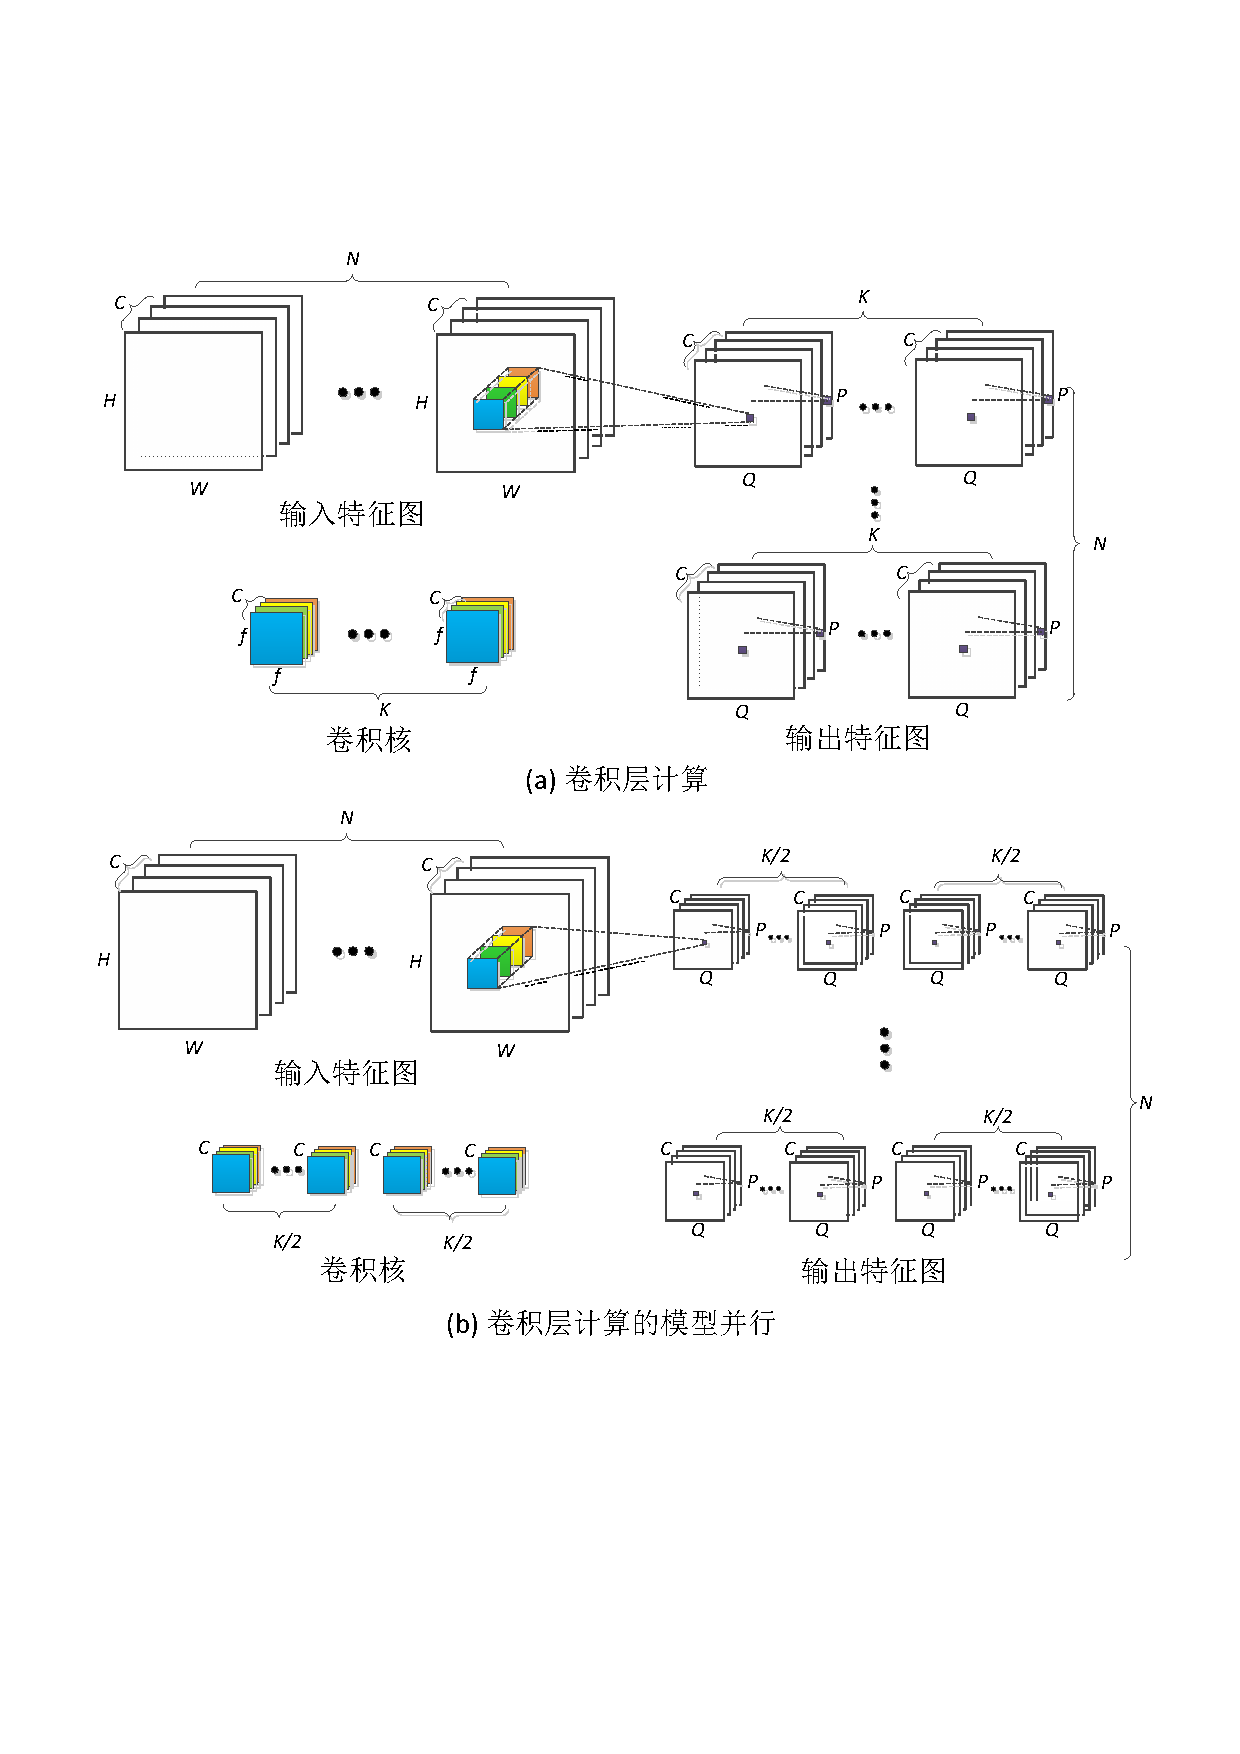
\includegraphics[width=12cm]{figs/ModelParallel.pdf}
%}
\caption{卷积层单GPU计算与双GPU的模型并行.}
\label{modelparallel}
\end{figure*}

对于通信阶段,可以采用的一种简单通信模式是选取一个计算设备作为主设备,在各个计算设备上的卷积计算完成后,
各个计算设备将计算的结果传输到主计算设备中,计算结果都汇总到主计算设备之后,由主计算设备再将汇总的结果分发到其它计算设备中。我们采用CUDA-Awared MPI,其算法实现如表\ref{simppleModelParallel}中的代码所示。

\begin{table}
\caption{基于多设备上的模型并行简单实现}
\label{simppleModelParallel}
\begin{lstlisting}[language=C++, basicstyle=\ttfamily\footnotesize]
void SimpleModelParallel( float* inputs,  float* weights,  float* outputs,  int N, int buf_size, int deviceNum, int kernel_stride, int output_stride... )
{
	...
	int my_rank;
	MPI_Comm_rank(MPI_COMM_WORLD, &my_rank);
	convComp(inputs, weights+my_rank*kernel_stride, outputs+my_rank*output_stride);
	if(my_rank==0){
		for(int i=1; i<deviceNum; i++)
			MPI_Recv(outputs+i*stride, buf_size, MPI_FLOAT, i, 0, MPI_COMM_WORLD );
	}
	else
		MPI_Send(outputs+i*stride, buf_size, MPI_FLOAT, 0, 0, MPI_COMM_WORLD);
	MPI_Bariier(MPI_COMM_WORLD);
	
	MPI_Broadcast(outputs, buf_size*deviceNum, MPI_FLOAT, 0, MPI_COMM_WORLD);
	...
}
\end{lstlisting}
\end{table}

下面从理论上分析单设备上卷积计算开销和多设备模型并行情况下时间开销。根据之前的假设,输入规模为$N\times H\times W\times C$,卷积核参数规模$C\times f\times f\times K$,输出规模为$N\times P\times Q\times K$,卷积核大小为$r$,单设备的峰值计算性能为$Peak$,单设备情形下的利用率为$\alpha$,总的计算量可以用如下公式表示:
\begin{equation}
L_1 = 2NPQCKr^2
\end{equation}

根据单设备计算能力以及利用率的假定,我们可以估算出单设备上卷积计算的时间$T_1$为:
\begin{equation}
T_1 = \frac{L_1}{\alpha \times Peak} = \frac{2NPQCKr^2}{\alpha \times Peak}
\end{equation}

在模型并行中,假设各个设备的利用率为$\beta$,计算设备数量为 $n$ ,则模型并行中的计算时间$T_2$为:
\begin{equation}
T_2 = \frac{L_1}{n \times \beta \times Peak} = \frac{2NPQCKr^2}{n\times \beta \times Peak}
\end{equation}

下面再计算模型并行中通信的时间开销,假定设备之间的通信带宽用$B$表示,则根据表\ref{simppleModelParallel}中算法描述的通信模式,可以计算出需要通信的数据总量$M$为:
\begin{equation}
M = \frac{NPQKr^2}{n}\times (n-1)+nNPQKr^2
\end{equation}

通信时间$T_3$为:
\begin{equation}
T_3 = \frac{M}{B} = \frac{\frac{NPQKr^2}{n}\times (n-1)+nNPQKr^2}{B}
\end{equation}

所以模型并行中的总时间$T_4$为:
\begin{equation}
\label{modelParallelTime}
T_4 = T_2 + T_3 = \frac{2NPQCKr^2}{n\times \beta \times Peak}+ \frac{\frac{NPQKr^2}{n}\times (n-1)+nNPQKr^2}{B}
\end{equation}

从\ref{modelParallelTime}中可以分析出,随着计算设备的数目$n$的增大,虽然计算时间会降低,但通信时间会增加,因此有必要对通信部分进行优化。\ref{commMode}将对通信模式进行优化,使得通信开销不会随着计算设备数目的增加而增大。

\subsection{优化的通信模式设计}
\label{commMode}
上一节中介绍的这种先收集到一个节点合并数据,然后再将数据广播到其它所有节点的方法并不是很高效的通信模式,本节将设计一种环形的拓扑结构进行通信,这种通信结构的特点是通信开销不会随着计算设备数目的增加而增大。

基于环形拓扑结构的通信只发生在相邻的计算节点间,通过多次相邻节点间的通信可以完成数据的收集与广播的目的。下面对通信的过程进行描述,每个计算设备存储部分计算结果,对计算设备进行从1到$n$进行编号,并且这$n$个计算设备按照环形的结构在逻辑上相连。数据的通信分$n$次完成,在第$i$次通信时,编号为$j$的计算节点将第$(i-1)$次接收的数据发送给编号为 $(j+1)\%n$的计算节点,同时从编号为$(j-1)\%n$的计算节点接收数据。在$n$次通信完成后,每个计算设备上最终的数据就是通信前各个计算设备上数据的拼接。图\ref{allgather}为计算设备数目为4时的通信过程示意图,具体的代码实现如表\ref{ringAllgatherA}中所示。

\begin{figure*}[tbh]%\small
\centering
\resizebox{0.8\textwidth}{!}{
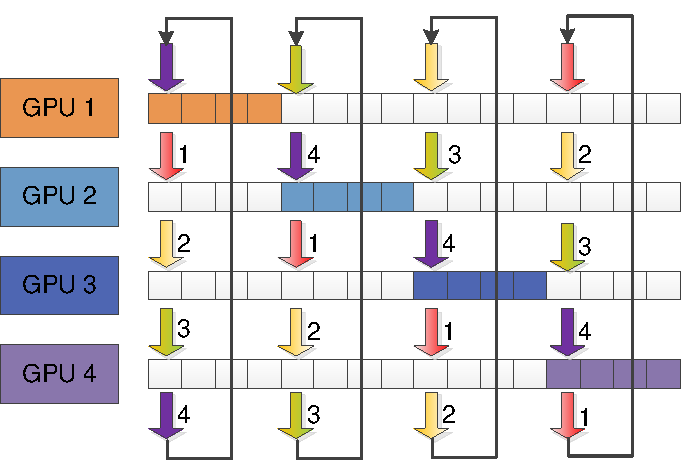
\includegraphics{figs/allgather.pdf}
}
\caption{基于环形拓扑结构下的4个GPU间数据交换示意图。每个GPU只与其邻居交换数据,allgather操作通过4次通信完成。}
\label{allgather}
\end{figure*}

\begin{table}
\caption{环形通信模式实现}
\label{ringAllgatherA}
\begin{lstlisting}[language=C++, basicstyle=\ttfamily\footnotesize]
void RingAllgather( float* outputs,  int buf_size, int deviceNum, int my_rank... )
{
	...
	int commNum = deviceNum;
	int send_to = (my_rank+1)\%deviceNum;
	int recv_from = (my_rank-1+deviceNum)\%deviceNum;
	float *send_buf, *recv_buf;
	send_buf = outputs+my_rank*buf_size;
	recv_buf = outputs+recv_from*buf_size;
	for(int i=0;i<commNum;i++){	
		for(int j=0;j<deviceNum;j++){
			MPI_Send(send_buf, buf_size, MPI_FLOAT, send_to, 0, MPI_COMM_WORLD);
			MPI_Recv(recv_buf, buf_size, MPI_FLOAT, recv_from, 0, MPI_COMM_WORLD);
		}
		send_buf = recv_buf;
		recv_buf = outputs+((i-1+deviceNum)\%deviceNum)*buf_size;
	}
	...
}
\end{lstlisting}
\end{table}

基于环形通信算法,下面对该算法的通信开销进行理论上的计算与分析。每个计算设备上需要交换的数据大小记为$M$,计算设备的数目记为$N$,设备$i$与相邻的通信设备$(i+1)\%N$间的通信带宽为$B_i$。则通过公式\ref{commT}可计算出总的通信开销$T$。

\begin{equation}
\label{commT}
T = N*\max_{i \in N}{\dfrac{M}{B_i}} = \max_{i \in N}{\dfrac{N\times M}{B_i}} = \max_{i \in N}{\dfrac{S}{B_i}}
\end{equation}

$S$代表从所有的计算设备收集汇总的数据,$S$一般是一个固定值,所以环形通信开销取决所有相邻节点间最小的通信带宽,而与通信的数据量无关,也与计算设备的数目无关。

\subsection{模型并行的流水化实现}
GPU支持kernel执行与数据传输并发的执行,所以我们可以进一步对通信进行优化,在通信进行的同时进行计算,这样可以隐藏通信的开销。由于通信与计算有相关性,即只有计算完成后,计算结果才能被用于通信,所以为了隐藏通信,需要将计算切分成多个阶段完成。GPU依次对切分的任务进行计算,对第$(i+1)$个任务的计算可以与第$i$次计算任务的结果的通信同时执行,这个方法就是模型并行的流水化执行。图\ref{pipelinedModelParallel}为多设备模型并行的流水化与多设备模型并行的简单实现以及单设备计算的比较示意图,对于模型并行流水化的理想实现中,大部分通信时间都得到了隐藏,只有最后一次计算结果的传输时间不能被隐藏,所以,理想情况下,应该提高计算划分的粒度,粒度越细,最后不能隐藏的通信时间越短。但在具体的实现中,卷积计算粒度并不是越细越好,因为计算被划分得越细,各个计算子任务变得越轻,导致GPU计算设备利用率下降,从而延长各个计算子任务的执行时间,这需要通过实验得到最佳的任务划分粒度。

\begin{figure*}[tbh]%\small
\centering
\resizebox{0.8\textwidth}{!}{
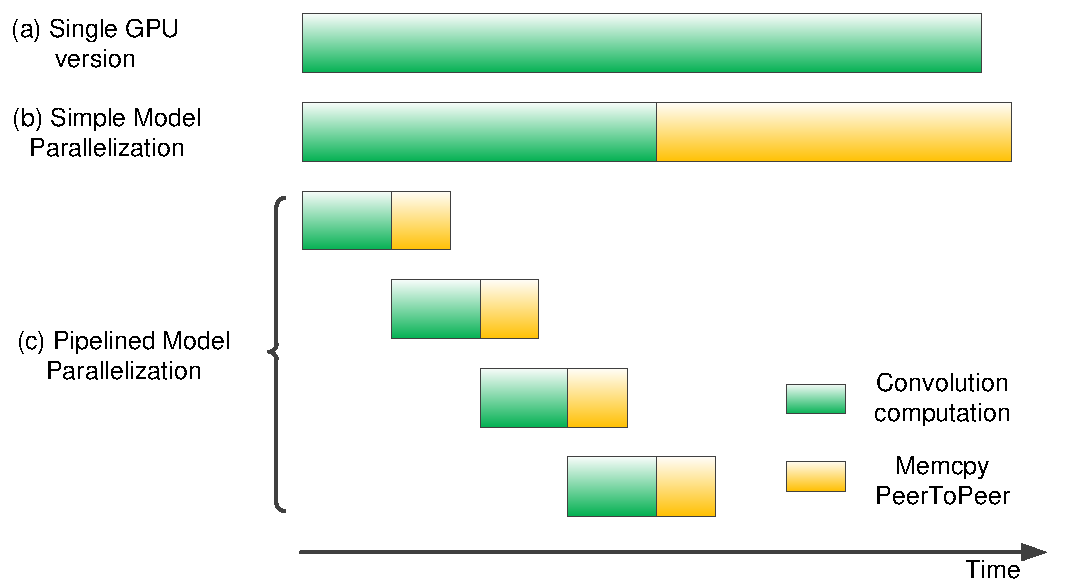
\includegraphics{figs/pipelinedModel.pdf}
}
\caption{三种实现方法下的时间分布:(a)单GPU实现,(b)简单模型并行版本,(c)流水化的模型并行}
\label{pipelinedModelParallel}
\end{figure*}

对于算法的具体实现,本工作采用的平台是Nvidia GPU,采用CUDA-Awared MPI编程,CUDA-Awared MPI提供异步的通信方式,而对于kernel的计算,CUDA提供事件方式进行控制,这为计算与通信重叠的实现提供了很好的基础。模型并行的流水化实现中,首先是为计算设备上的所有计算任务创建一个事件进行关联,其次将所有的计算kernel压入命令队列中等待GPU执行,然后依次查询各个计算kernel关联的时间,看计算任务是否完成,如果计算完成,则可以对已经完成的计算任务的计算结果进行通信。表\ref{OverlapA}中是具体的算法实现。

\begin{table}
\caption{模型并行流水化的代码实现}
\label{OverlapA}
\begin{lstlisting}[language=C++, basicstyle=\ttfamily\footnotesize]
void PipelinedModelParallel( float *inputs, float *filters, float* outputs,  int delta_num, int buf_size, int deviceNum, int stride1, int stride2... )
{
	...
	int my_rank;
	MPI_Comm_rank(MPI_COMM_WORLD, &my_rank);
	stream_t streamT[delta_num];
	int commNum = deviceNum;
	int send_to = (my_rank+1)\%deviceNum;
	int recv_from = (my_rank-1+deviceNum)\%deviceNum;
	float *send_buf, *recv_buf;
	send_buf = outputs+my_rank*buf_size;
	recv_buf = outputs+recv_from*buf_size;
	for(int i=0; i<delta_num; i++){
		cudaStreamCreate(streamT[i]);
		convComp(inputs, filters+i*stride2, outputs+my_rank*stride1+i*stride2, streamT[i]);
	}
	for(int j=0; j<delta_num; j++){
		cudaStreamSynchronize(streamT[j]);
		send_buf = outputs+my_rank*stride1+j*stride2;
		recv_buf = outputs+recv_from*stride1+j*stride2;
		for(int i=0;i<commNum;i++){	
			for(int j=0;j<deviceNum;j++){
				MPI_Send(send_buf, buf_size, MPI_FLOAT, send_to, 0, MPI_COMM_WORLD);
				MPI_Recv(recv_buf, buf_size, MPI_FLOAT, recv_from, 0, MPI_COMM_WORLD);
			}
			send_buf = recv_buf;
			recv_buf = outputs+((i-1+deviceNum)\%deviceNum)*stride1+j*stride2;
		}
	}
	...
}
\end{lstlisting}
\end{table}

\section{实验评测与分析}
本节对两个常用的2D以及3D卷积网络的模型并行实现进行了评测与分析,比较了多设备上模型并行性能与单设备上的性能,并且比较了模型并行简单实现的性能与模型并行的流水化实现的性能。

\subsection{实验设置}
所有实验都在带有2个Nvidia K20 GPU的服务器上做的测试,K20是Keple体系结构,支持GPU Direct技术。实验的软件环境包括CUDA 8.0, cudnn 5.0以及OpenMP。每个卷积计算将调用cudnn库,GPU间的数据通信使用CUDA-Awared MPI。

\subsection{2D卷积层的模型并行实现的性能}
本实验选取了一个常用的2D卷积神经网络即VGG网络,该神经网络包含多层卷积层,这些卷积层涵盖了主要的计算,所以本章介绍的模型并行主要用于加速卷积层的计算,从而降低卷积神经网络前向计算过程的延迟。第一个实验比较了VGG网络的各个卷积层在单GPU上实现的性能与多GPU上模型并行简单实现的性能。单GPU上的实现只包含计算时间,而多GPU上的模型并行的简单实现包含计算和GPU间的通信。

图\ref{singleAndSimple}为VGG网络前向计算过程单GPU实现与多GPU模型并行简单实现的性能比较。实验测试了VGG卷积网络的所有卷积层的前向计算的执行时间,从实验结果可以看到,除了第一层卷积层,其它卷积层的多GPU实现性能都比单GPU上实现性能好,在多GPU实验中使用的是2个GPU,理论上来说2个GPU上的模型并行性能应该是单GPU上性能的2倍,但在实验中,取得最好加速效果的应该是$conv3 \_2$,相比单GPU性能,双GPU性能提高了约45\%。对于VGG网络的前面几层以及最后一层卷积层,提升的效果就不是特别明显了(比如卷积层$conv1\_2$、$conv2\_1$、$conv2\_2$、$conv5\_1$),有的甚至性能下降了(如$conv1\_1$),这是因为对于VGG卷积网络的开始的卷积层,卷积层输入的通道数都还比较少,卷积核的输出通道数也比较少,所以这些卷积层的计算量并不大,对于单GPU来说,都很难发挥单GPU的效率,而在多GPU的模型并行中,还需要将少量的计算进一步划分到各个GPU上,则多GPU上效率比单GPU上的效率更低,因此,双GPU上的执行时间与单GPU相比,并不能达到理想的一半的效果,并且在开始的卷积层的输入输出分辨率往往比较大,所以输出特征图所需的存储也相对较大,多GPU上的通信开销将比较大。在第一层卷积层,这两个问题尤为突出,因此我们看到最后单GPU上的性能超过了双GPU模型并行的性能。

\begin{figure*}[tbh]%\small
\centering
\resizebox{0.8\textwidth}{!}{
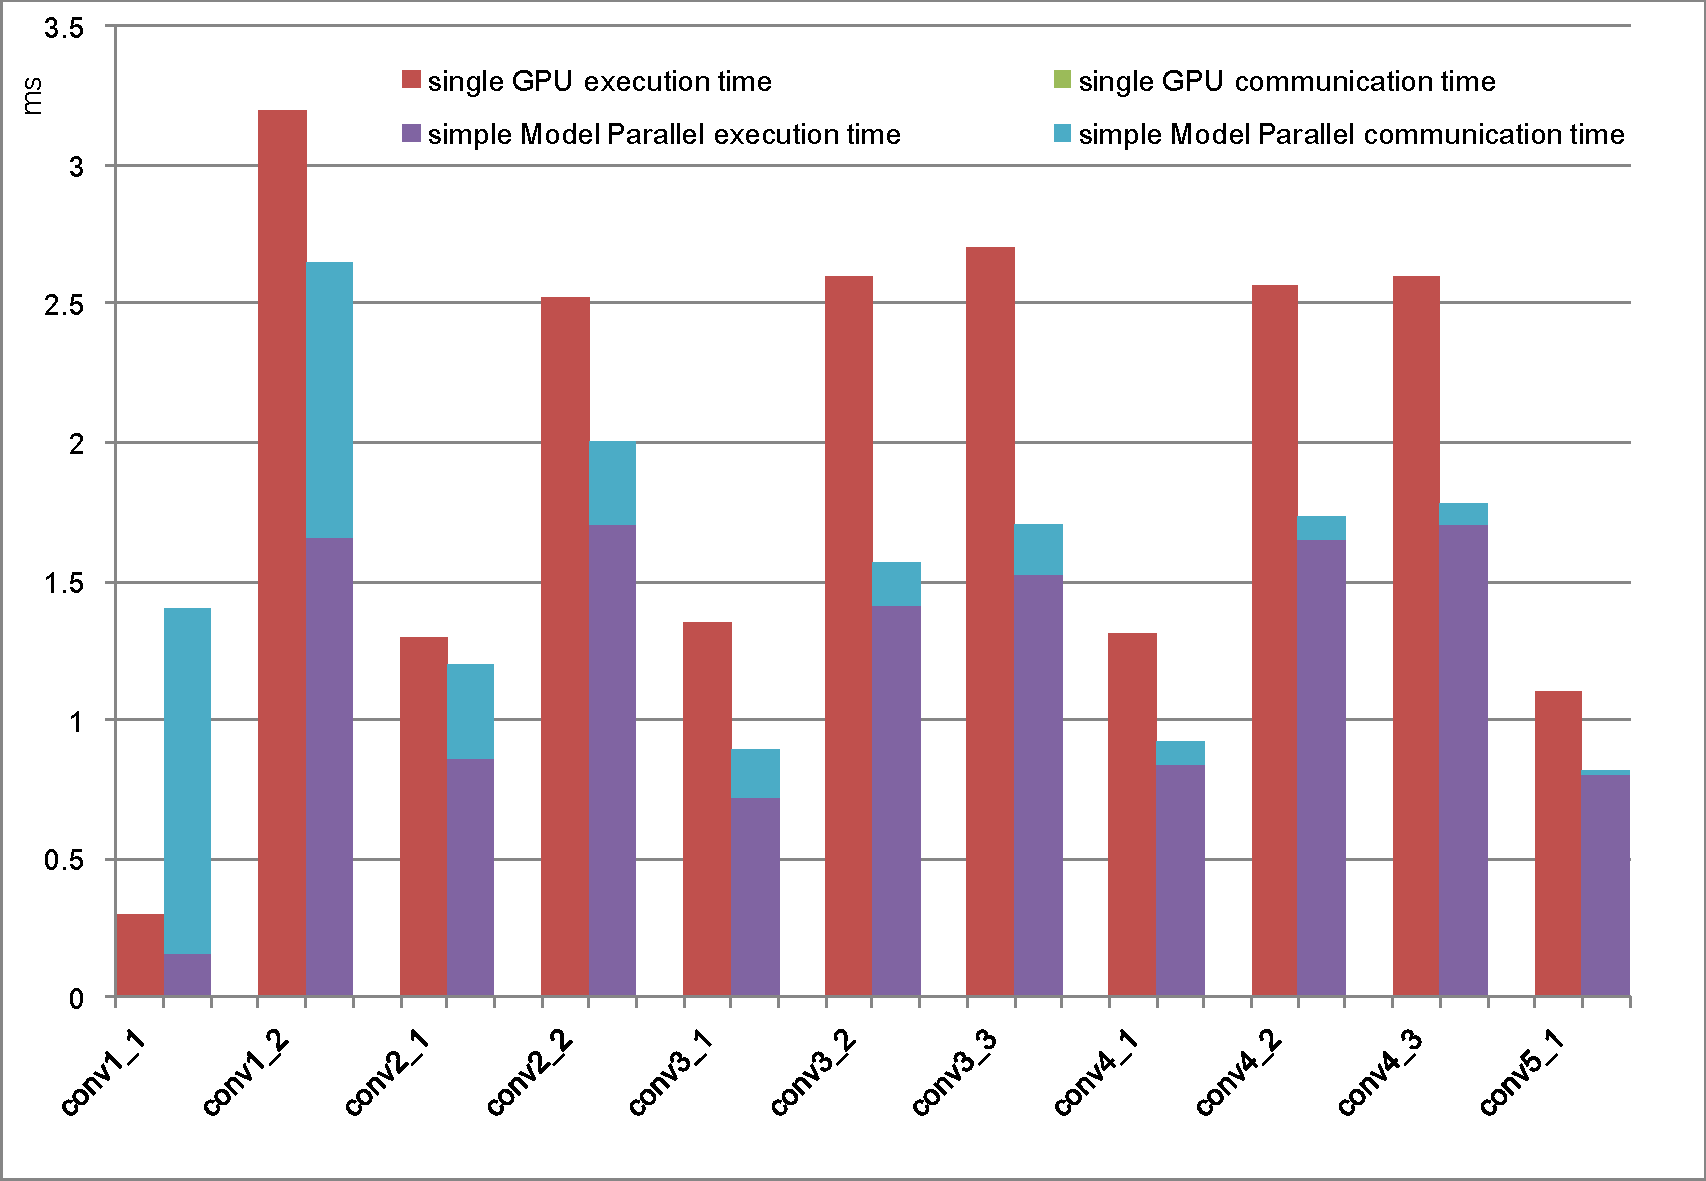
\includegraphics{figs/singleAndSimple.pdf}
}
\caption{2D卷积网络的单GPU实现以及简单模型并行实现的性能。}
\label{singleAndSimple}
\end{figure*}

从第一个实验中,我们可以看出模型并行的简单实现存在的问题,一个是由于模型并行导致计算负载过轻而影响GPU效率的发挥,二是通信开销没有得到隐藏。第二个实验是对模型并行流水化的性能评测,模型并行的流水化可以使得通信得到隐藏,但并不能解决模型并行中效率低下的问题,而且由于模型并行的流水化中计算被切成更多小的计算任务,这个效率低下的问题会更加严重,为此在模型并行的流水化中,引入了Nvidia GPU中提供的并发kernel执行的技术。所以在第二个实验中,测试了模型并行的简单实现的性能、模型并行流水化而未采用kernel并发执行技术的性能以及模型并行流水化并且采用了kernel并发执行技术的性能。测试的对象仍然是VGG网络的所有卷积层,图\ref{simpleAndPipelined}为实验结果。单从比较通信时间可以发现,模型并行的流水化的两种实现中通信时间都比模型并行的简单实现少,所以模型并行的流水化方法确实能达到隐藏通信的目的。而比较这三种实现的总时间会发现,模型并行的流水化中未采用并发技术的时间都要比另两种方法长,这是因为模型并行的流水化而未采用并发技术的实现中GPU利用率低,使得计算部分的总时间明显比模型并行的简单实现中的计算时间长。而在采用了并发技术之后,我们可以观察到模型并行的流水化在某些卷积层(如$conv2\_1$、$conv2\_2$)最后总的时间要比模型并行的简单实现的时间短。而对于其它层,主要是这些卷积层的kernel实现中,线程块数目足够大,使得并发技术并没有完全发挥出效果。

\begin{figure*}[tbh]%\small
\centering
\resizebox{0.8\textwidth}{!}{
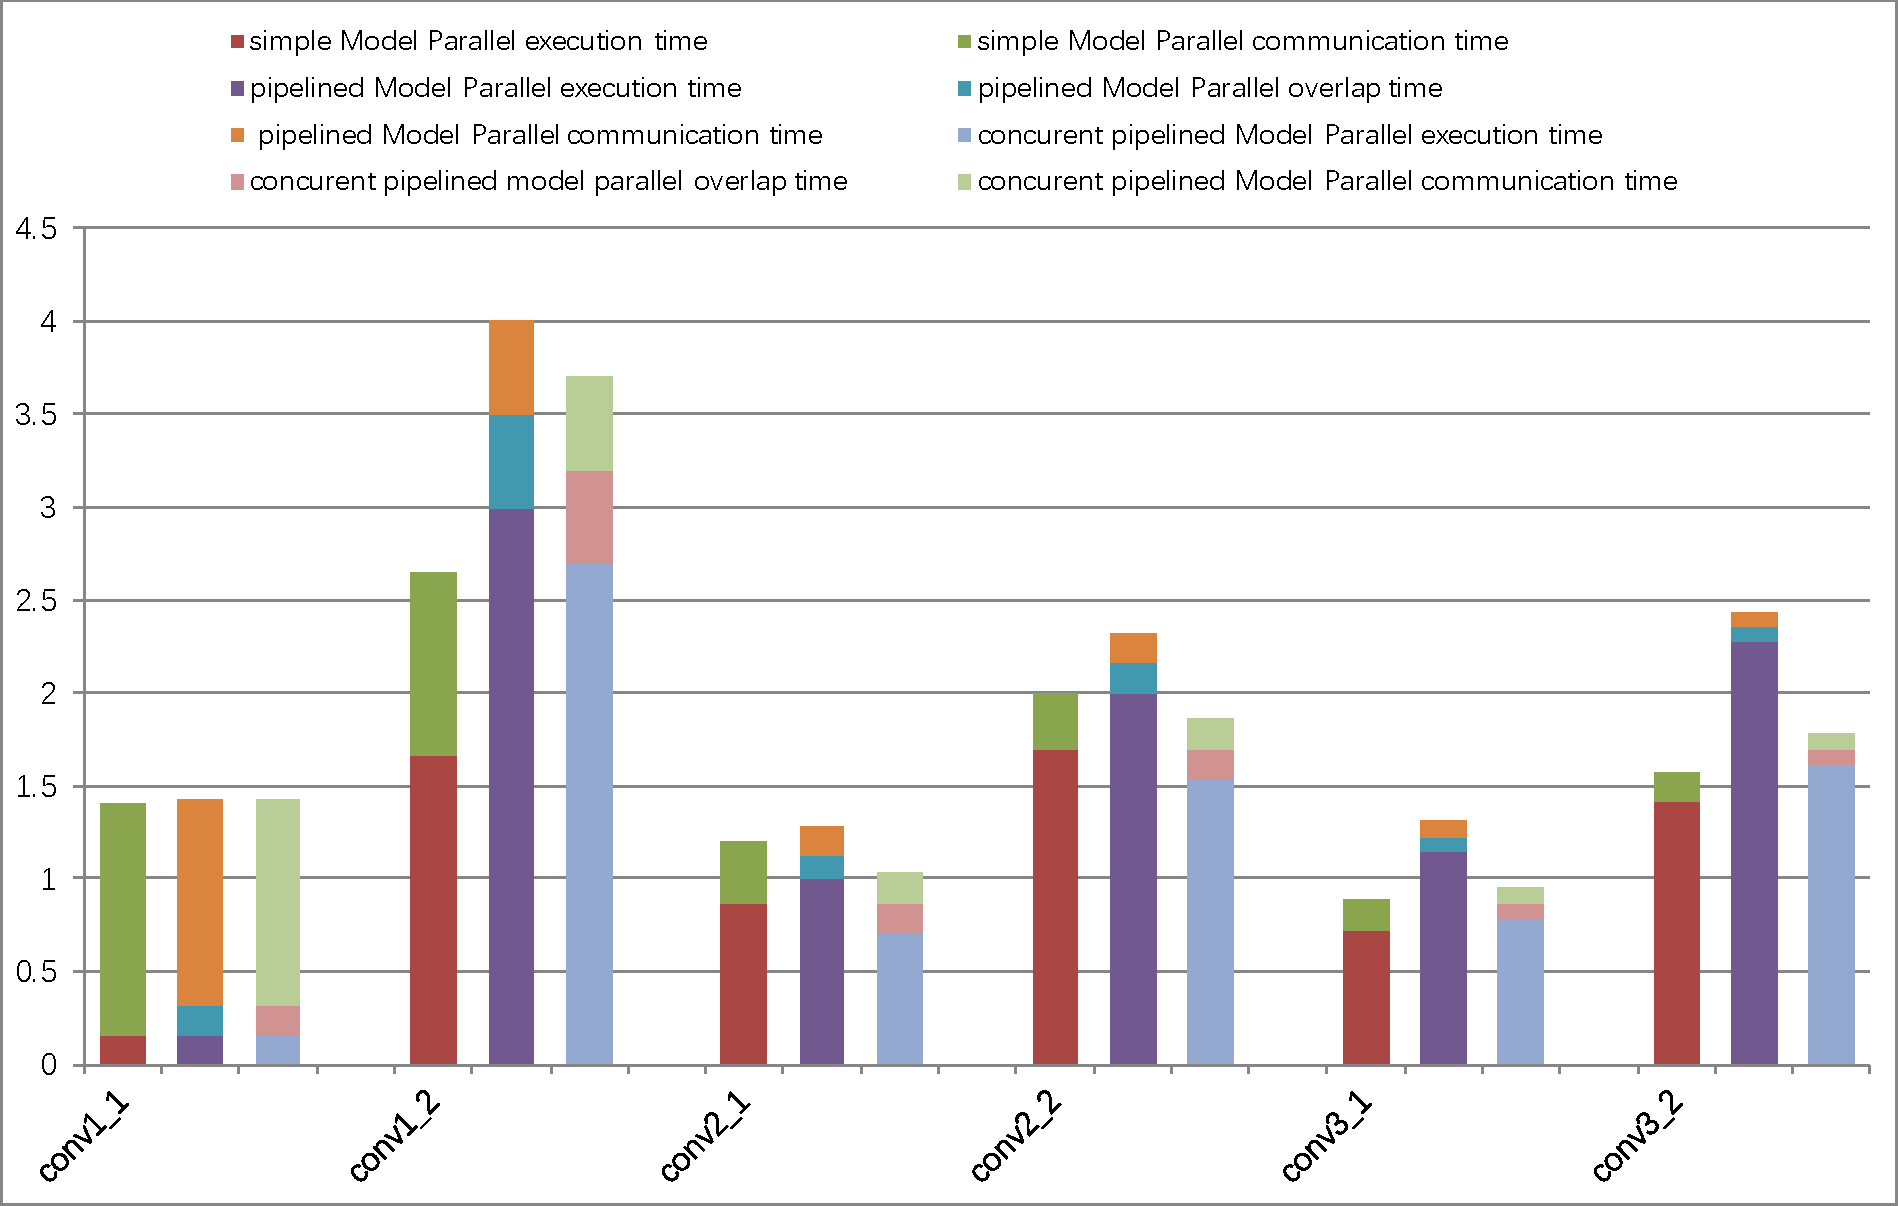
\includegraphics{figs/simpleAndPipelined.pdf}
}
\caption{2D卷积层的简单模型并行以及流水化的模型并行的各计算部分的时间开销分布。}
\label{simpleAndPipelined}
\end{figure*}

\subsection{3D卷积层模型并行实现性能}
模型并行同样可以应用到3D卷积神经网络中,在本节实验中,主要测试一个用于视频分析的3D卷积神经网络,这个3D卷积神经网络名为C3D,在C3D中,有5层卷积层,表\ref{conv3d-info}为该3D卷积神经网络各个卷积层的参数配置。

\begin{table}[]
\centering
\caption{3D卷积网络的卷积层信息,其中卷积核大小为$3\times 3\times 3$,batch大小为$1$。}
\label{conv3d-info}
\begin{tabular}{|c|c|c|c|}
\hline
Layer & CxDxHxWxN       & K   \\ \hline
conv1 & 3x16x112x112x1 & 32   \\ \hline
conv2 & 32x16x56x56x1  & 64   \\ \hline
conv3 & 64x8x28x28x1   & 256  \\ \hline
conv4 & 256x4x14x14x1  & 256  \\ \hline
conv5 & 256x2x7x7x1    & 256  \\ \hline
\end{tabular}
\end{table} 

本节实验比较了3D卷积神经网络的单GPU实现、双GPU的模型并行的简单实现以及双GPU的模型并行的流水化实现。图\ref{3DSimpleAndPipelined}为C3D网络的各个卷积层的这三种实现的总时间比较。与2D卷积层类似,对于大部分3D卷积层来说,它们的双GPU的模型并行的简单实现可以取得一定的加速效果,与单GPU的实现性能相比,双GPU的模型并行的简单实现可以提高$20\%\sim40\%$的性能。在卷积层$conv1$,模型并行实现的性能反而下降了,其原因也是因为在第一层卷积层中,计算量太小,导致模型并行中GPU计算效率明显下降,而输出特征图相对较大,又导致模型并行中的通信开销增加。最终使得模型并行实现的性能低于单设备的实现。

在模型并行的流水化实现中,除了卷积层$conv5$,其它层的执行时间并没有比模型并行的简单实现少,其中主要的原因为C3D的设计上为了控制计算量,各个卷积层的输入输出通道数较小,特征图大小也因为抽样分辨率下降明显,所以各个卷积层在GPU上实现时,cuDNN库中所使用的线程块大小以及线程块内的线程数都较小,使得模型并行的流水化实现中并发技术并不能明显提高GPU的利用效率,流水化实现带来的通信隐藏并不能弥补由于GPU效率下降而损失的性能。本章介绍的模型并行流水化技术适合计算量巨大的卷积层,因为只有那些计算量巨大的卷积层,被切分之后的子任务才具备足够的计算量提高GPU硬件资源的利用率,模型并行流水化的计算总时间才能有效降低。

\begin{figure*}[tbh]%\small
\centering
\resizebox{0.8\textwidth}{!}{
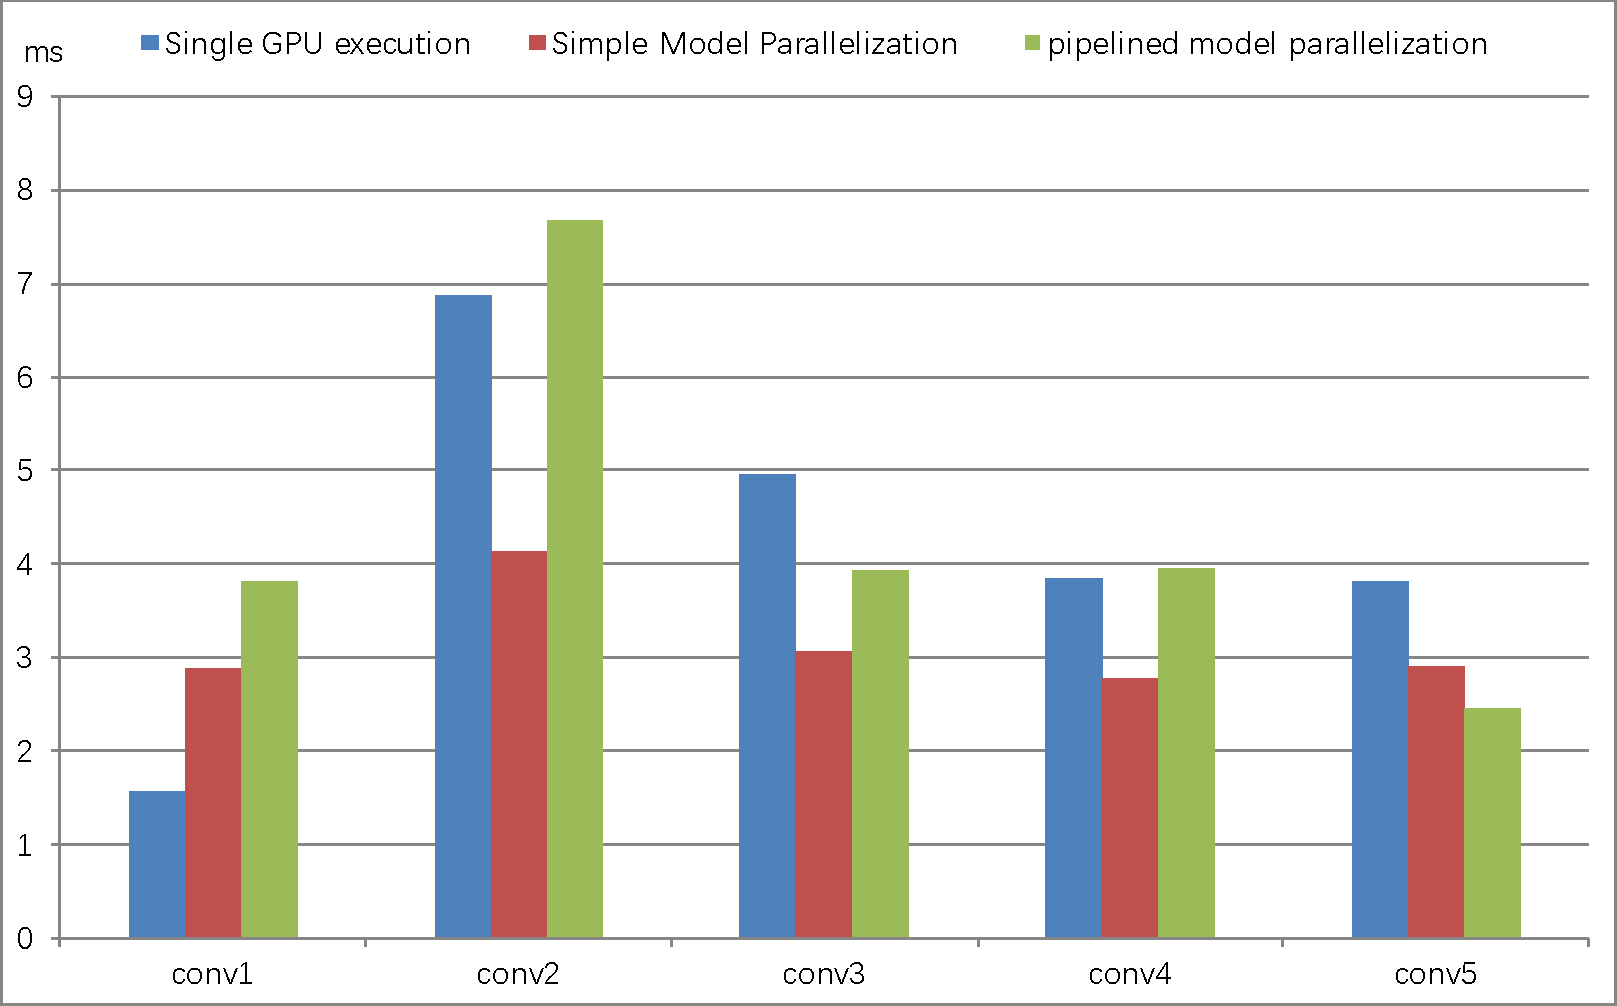
\includegraphics{figs/3DSimpleAndPipelined.pdf}
}
\caption{3D卷积网络的单GPU实现,简单并行实现以及流水化的模型并行实现的性能比较。}
\label{3DSimpleAndPipelined}
\end{figure*}

\section{小结}
本章主要介绍了在数据中心环境下,针对卷积神经网络应用而提出的一个低延迟的解决方案,采用模型并行的方法在多个计算设备上进行并行加速。介绍了多个计算设备上的模型并行的简单实现,相比于单设备上的卷积实现,卷积计算部分在多个计算设备上确实得到了加速的效果,但存在的问题是模型并行中存在很大比重的通信开销,而且通信开销随着计算节点的数目增加而变得复杂。针对模型并行简单实现中通信开销上存在的问题,本章介绍了一种环形结构的通信模式,这种环形结构的通信模式的通过将需要交换的数据切分成小段数据,每个计算设备只向邻居设备发送数据和接收数据,数据链路构成一个环形结构,每个设备只需要与相邻的设备通信,这有效降低了通信的复杂度,而且最终的通信开销只取决于相邻设备间带宽最小的链路,与需要通信的设备数目无关。为了进一步隐藏通信开销,本章介绍了模型并行的流水化实现,即将卷积计算划分成很多小的计算任务,然后将计算和通信交替执行,进而达到计算与通信重叠的目的,对于计算量小的卷积层,模型并行流水化虽然能隐藏大部分通信时间,但会造成计算设备计算效率降低,从而增大计算的总时间,对于GPU设备来说,本章介绍的kernel并发技术在一定程度上可以缓解GPU设备效率低的问题。

最后从实验结果来看,模型并行的多种实现中计算部分的时间加速并不能达到理想的效果,主要是各层卷积层的计算量还不够,特别是模型并行的流水化实现中,由于计算任务被划成更多小的计算任务,多计算设备上的利用效率更低了。即使采用GPU中的kernel并发执行机制,也只能对某些卷积层有效。但如果只从通信开销来看,模型并行的流水化实现中确实达到了计算与通信重叠的目的,通信时间得到了有效隐藏。

可以预测,对于未来计算更加密集型的卷积神经网络的前向计算过程,本章介绍的技术将达到更好的效果。






